\documentclass[a4j]{jarticle}
\usepackage{graphicx}
\usepackage[left=25truemm,right=25truemm]{geometry}

\title{画像処理 レポート}

\author{氏名: 木下直樹\\学籍番号: 09425521}

\begin{document}
\maketitle

%%%%%%%%%%%%%%%%%%%%%%%%%%%%%%%%%%%%%%%%%%%%%%%%%%
\section{概要}
%%%%%%%%%%%%%%%%%%%%%%%%%%%%%%%%%%%%%%%%%%%%%%%%%%
第6回の実験ではTKfilter.cで得られた二つの画像の特徴点を対応付けするプログラムを作成した. 
今回はそのプログラムから得られた特徴点セットから4セットを選び, 二つの画像を合成するのに適切な射影行列を計算するプログラムを作成する. 
どの4点を選ぶとよいかを判断することは難しいので, ランダムに選んだ4点で行列の適正を計算することを繰り返して最も適した行列を採用する.

%%%%%%%%%%%%%%%%%%%%%%%%%%%%%%%%%%%%%%%%%%%%%%%%%%
\section{課題}
%%%%%%%%%%%%%%%%%%%%%%%%%%%%%%%%%%%%%%%%%%%%%%%%%%
ファイルを新たに作成せずgreedy.cを拡張して射影行列の計算と選出を実装した. 
TKfilter.cから特徴点の対応セット30をファイルに出力し, そのファイルをgreedy.cで参照する形をとった. 
その対応点のセットから無作為に4つ拾うアルゴリズムは, 以下の様にした. 
\begin{enumerate}
\item 特徴点セットをすべてw[30][4]に格納する.
\item 0から29までの数が1つずつ格納された配列rndAry[30]の中の値を無作為に入れ替える. 
\item rndAry[0],rndAry[1],rndAry[2],rndAry[3]に格納された値を添字とする特徴点セットw[][]に格納された特徴点セットを採用する.
\end{enumerate}

選ばれた特徴点セットで射影行列を計算するが, これにより得られた射影行列は無作為に選ばれた特徴点によるものであるため, 適切な行列かどうかは判別ができない. そこで以下の様な計算で得られた値の大きさで判断する. 

\begin{enumerate}
\item w[][]に格納されたある特徴点セットをx,y,u,vとする
\item 一方の画像の特徴点座標x,yが画像の台形変換により他方の画像の特徴点座標u,vに近ければ制度の高い射影行列である可能性が高い
\item この座標x,yが変換後に移る座標と座標u,vの距離の2乗が一定の値より小さい場合カウントする
\item 30セット全てにこの操作をし, カウントした値を返す
\item この値の数が大きいほど使用した射影行列が適切であったことの証明となる
\end{enumerate}

以上の様な操作を次の様な手順でより最適な射影行列を計算する.

\begin{enumerate}
\item 対応付けられた特徴点から無作為に4セット選出する
\item それらから射影行列を計算する
\item 得られた射影行列の適正を図る
\item 得られたカウントがこれより前に得られたものより大きければこの射影行列を保持する
\item 指定した回数以上を繰り返し, 最も適した射影行列を出力する
\end{enumerate}

上記の手順が今回拡張したgreedy.cの中身になる.
また, 上記の通り, このプログラムではlsq.cの射影行列計算を頻繁に実行するため, lsq.c内のmain関数の関数名をLSQに変更し, greedy.cから使用できるように仕様の変更をした. 

得られた射影行列を用いて0.jpgと2.jpgを合成した画像は次のようになった.


\begin{figure}[b]
\begin{center}
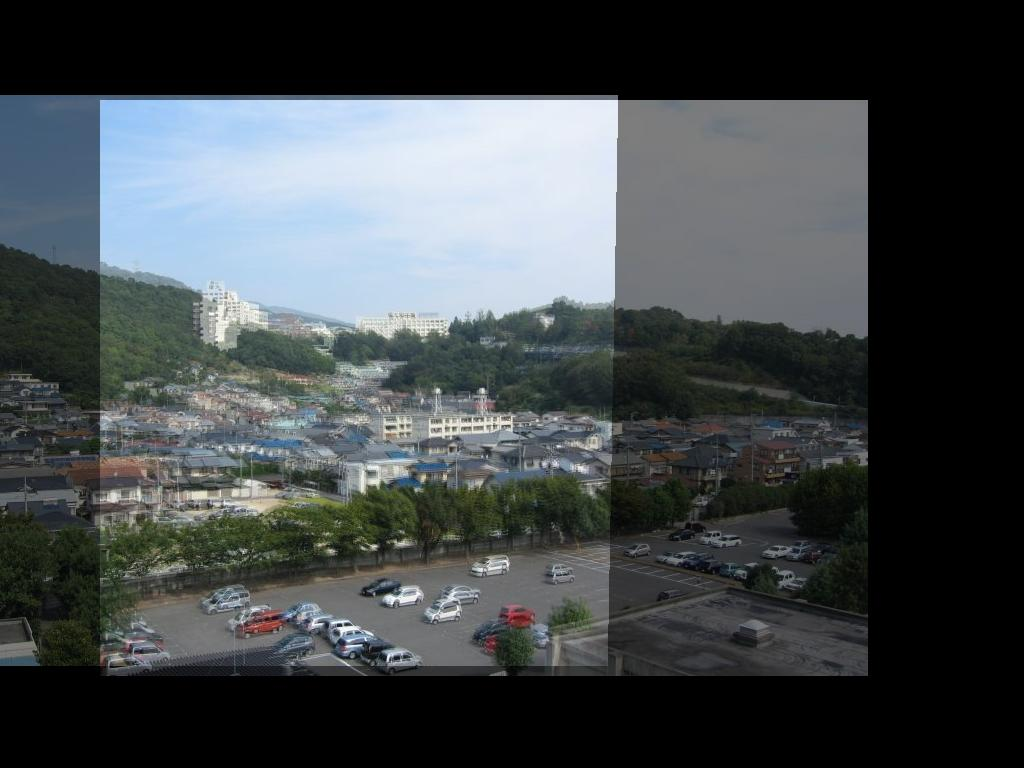
\includegraphics[bb=0 0 768 576,scale=.3]{out.jpg}
\caption{0.jpgと2.jpgの合成}
\end{center}
\end{figure}



\end{document}
